\chapter{Background}
\label{chap:background}
This chapter introduces the concepts on which the rest of the thesis builds.
The problem studied here draws on several fields. Process mining provides the
data model, event logs and traces, and predictive and prescriptive process
monitoring turn a running trace into a recommendation. Multi-objective
optimization frames the trade-off between conflicting KPIs. Gradient boosting
provides the predictions, and quantifying its uncertainty is the core of this
work. Business process simulation, finally, is used to evaluate the
recommendations.

\section{Process Mining: Basic Concepts}
\label{sec:bg:pm}
Process mining is a discipline that combines data science and process
management: it analyzes the data recorded by information systems to
reconstruct how business processes actually run. Every execution of a
process, such as the handling of a reimbursement request, leaves traces in
the systems that support it, in the form of event logs that record which
activity was performed, when, and for which case. From these logs, process
mining techniques discover the process model as it is actually executed,
check its conformance to an expected model to find deviations, and enhance
it with further information useful for improving the
process~\cite{vanderaalst2016}.

    \subsection{Event Log, Traces, Events}
    \label{subsec:bg:pm:log}
    The starting point of any process-mining analysis is the \emph{event log}. An
    event log $\mathcal{L}$ collects the executions of a business process, called
    \emph{traces}: each trace $\sigma = \langle e_1, e_2, \dots, e_n \rangle$ is a
    chronologically ordered sequence of events produced by one instance (or case)
    of the process, and $|\sigma|$ denotes its length. Every event
    $e = (c, a, \mathbf{d})$ is uniquely tied to a trace through a case identifier
    $c$, records the execution of one activity $a$, and carries a vector of
    additional attributes $\mathbf{d}$ such as the start
    and completion timestamps of the activity and the resource that performed
    it~\cite{le2025balancing}. Table~\ref{tab:bg:pm:log} shows a small event
    log of three cases.

    \begin{table}[h]
      \centering
      \small
      \begin{tabular}{cccll}
        \toprule
        Case & Activity & Resource & Start & Completion \\
        \midrule
        $c_1$ & $a$ & $r_1$ & Mar 4, 09:12 & Mar 4, 09:30 \\
        $c_1$ & $b$ & $r_2$ & Mar 4, 10:05 & Mar 4, 11:20 \\
        $c_1$ & $c$ & $r_3$ & Mar 5, 08:40 & Mar 5, 09:15 \\
        $c_1$ & $d$ & $r_2$ & Mar 5, 14:00 & Mar 5, 14:45 \\
        \midrule
        $c_2$ & $a$ & $r_1$ & Mar 4, 09:40 & Mar 4, 09:55 \\
        $c_2$ & $c$ & $r_3$ & Mar 4, 13:10 & Mar 4, 13:50 \\
        $c_2$ & $e$ & $r_4$ & Mar 6, 10:00 & Mar 6, 10:30 \\
        \midrule
        $c_3$ & $a$ & $r_1$ & Mar 5, 08:55 & Mar 5, 09:10 \\
        $c_3$ & $b$ & $r_2$ & Mar 5, 11:00 & Mar 5, 12:10 \\
        $c_3$ & $c$ & $r_3$ & Mar 6, 09:00 & Mar 6, 09:40 \\
        $c_3$ & $e$ & $r_4$ & Mar 7, 15:20 & Mar 7, 15:35 \\
        \bottomrule
      \end{tabular}
      \caption{An event log of three cases. Each row is an event
        $e = (c, a, \mathbf{d})$, whose attributes $\mathbf{d}$ are the
        resource and the start and completion timestamps. Ordering each case's
        events by time gives the traces $\langle a,b,c,d\rangle$,
        $\langle a,c,e\rangle$ and $\langle a,b,c,e\rangle$, the log
        $\mathcal{L}^{\mathrm{ex}}$ of Figure~\ref{fig:bg:pm:ts}.}
      \label{tab:bg:pm:log}
    \end{table}

    The sets $\mathcal{A}$ and $\mathcal{R}$ contain, respectively, the activity
    labels and the resources that occur anywhere in the process;
    $\mathcal{E}$ is the universe of possible events and $\mathcal{E}^{*}$ the
    space of finite event sequences over it. Two projection functions,
    $act : \mathcal{E} \to \mathcal{A}$ and $res : \mathcal{E} \to \mathcal{R}$,
    extract the activity and the resource of an event. Because an activity can
    occur more than once along the same trace (e.g.\ inside a loop), ``event''
    and ``activity occurrence'' are the more precise terms, even though the
    shorter ``activity'' is used informally throughout whenever no ambiguity
    arises.

    \subsection{Prefixes and Running Traces}
    \label{subsec:bg:pm:prefix}
    A historical event log records completed traces, but at any given moment
    some cases of the process are still in progress and have executed only
    part of their events. Given a complete trace
    $\sigma$, its $k$-\emph{prefix} $\sigma_{(k)} = \langle e_1, \dots, e_k
    \rangle$, with $1 \le k \le |\sigma|$, is the sequence of its first $k$
    events~\cite{le2025balancing}. For $k < |\sigma|$, the
    remaining $\langle e_{k+1}, \dots, e_n \rangle$ is the suffix that has not
    happened yet. A \emph{running}, or ongoing, execution is exactly such a
    prefix with $k < |\sigma|$, produced by a case that has not reached
    completion.

    \subsection{State Abstraction and Transition Systems}
    \label{subsec:bg:pm:ts}
    A common way to reason about prefixes in process mining is a
    \emph{transition system}~\cite{vanderaalst2016}, a
    directed graph whose nodes are \emph{states} and whose edges are labeled
    with activities: an edge from state $s$ to state $s'$ labeled $a$ means
    that executing $a$ from $s$ leads to $s'$. States abstract prefixes
    through a state-representation function $S$, mapping every prefix
    $\sigma_{(k)}$ to some state $S(\sigma_{(k)})$; two prefixes that map to
    the same state are treated as equivalent, even if their histories differ.
    
    Given a log of completed traces $\mathcal{L}$, the transition system is
    mined by recording, for every state that occurs in the log, the
    activities empirically observed to follow it, each as an edge leaving
    that state.

    The choice of $S$ shapes the resulting transition system. Using the
    prefix itself as the state, $S(\sigma_{(k)}) = \sigma_{(k)}$, offers
    little help: a state would then correspond to one specific history, so
    nothing learned from one case would transfer to another, and the number
    of states would grow with every distinct prefix in the log. A common
    abstraction keeps only the last $w$ activities of the prefix, as in
    Figure~\ref{fig:bg:pm:ts}. The window $w$ decides how much recent history
    two prefixes must share to reach the same state.

    \begin{figure}[h]
      \centering
      \begin{tikzpicture}[
        >={Stealth[length=2mm]},
        state/.style={draw, rounded corners, minimum height=7mm, font=\small,
                      inner sep=3pt},
        lbl/.style={font=\scriptsize, inner sep=1.5pt}]
        \node[state] (s0) at (0,0)      {$\langle\,\rangle$};
        \node[state] (a)  at (2,0)      {$\langle a\rangle$};
        \node[state] (ab) at (4,0.9)    {$\langle a,b\rangle$};
        \node[state] (ac) at (4,-0.9)   {$\langle a,c\rangle$};
        \node[state] (bc) at (6.6,0.9)  {$\langle b,c\rangle$};
        \node[state] (cd) at (9.0,1.6)  {$\langle c,d\rangle$};
        \node[state] (ce) at (9.0,-0.6) {$\langle c,e\rangle$};
        \path[->]
          (s0) edge node[lbl,above]      {$a$} (a)
          (a)  edge node[lbl,above left] {$b$} (ab)
          (a)  edge node[lbl,below left] {$c$} (ac)
          (ab) edge node[lbl,above]      {$c$} (bc)
          (bc) edge node[lbl,above left] {$d$} (cd)
          (bc) edge node[lbl,left]       {$e$} (ce)
          (ac) edge node[lbl,below]      {$e$} (ce);
      \end{tikzpicture}
      \caption{Transition system mined from the toy log
        $\mathcal{L}^{\mathrm{ex}} = \{\langle a,b,c,d\rangle,\ \langle a,c,e\rangle,\
        \langle a,b,c,e\rangle\}$ with window $w = 2$. A state is the last two
        activities of a prefix; an edge records an activity observed to follow that
        state somewhere in the log. From $\langle b,c\rangle$ the log continues
        with $d$ or $e$, and any prefix reaching the same state inherits these
        continuations, even one never seen in full.}
      \label{fig:bg:pm:ts}
    \end{figure}

\section{Prescriptive Process Analytics}
\label{sec:bg:prpa}
Data analytics is commonly described as a progression of four questions of
increasing sophistication and business value~\cite{ibm_prescriptive}:
\begin{itemize}
    \item descriptive analytics asks what happened;
    \item diagnostic analytics asks why it happened;
    \item predictive analytics asks what is likely to happen next;
    \item prescriptive analytics asks what should be done next.
\end{itemize}
The four are complementary, each building on the output of the previous one.
Only the last recommends a course of action and makes the implications of
each option explicit~\cite{wikipedia_prescriptive}. To do so, prescriptive
analytics combines historical and contextual data with business rules and
with mathematical and computational models drawn from statistics, machine
learning and operations research, and reasons about objectives,
constraints, uncertainty and trade-offs at once. It is applied, for
example, to recommend a treatment from a patient's characteristics, to set
prices and plan promotions from a demand forecast, to schedule maintenance
before a machine fails, or to score a transaction for fraud
risk~\cite{ibm_prescriptive}.

When this paradigm is applied to the executions of a business process
recorded in an event log, it is called \emph{Prescriptive Process Analytics}
(PrPA), or prescriptive process monitoring~\cite{kubrak2022}. PrPA supports
\emph{ongoing} process executions by suggesting interventions that steer a
running case toward a desired result, for instance preventing an
unfavorable outcome or reducing the cost or the duration of the case.
Predictive process monitoring estimates a property of the running case,
such as its outcome, its remaining time or its most likely next activity;
prescriptive monitoring uses those estimates to decide which action
improves a target performance measure, taking the dependencies between the
different aspects of the process into account~\cite{lepenioti2020}.

The kind of action prescribed varies across the literature. Early work
recommended the next activity to execute by exploiting the event data payload
and simple counterfactual reasoning~\cite{groger2014}. As prediction-based
methods spread, attention moved to flagging cases at risk of an undesired
outcome and to deciding whether and when to
intervene~\cite{teinemaa2018,fahrenkrogpetersen2022}. More recent approaches
recommend how to proceed using causal inference~\cite{bozorgi2021prescriptive, bozorgi2023},
reinforcement learning~\cite{branchi2022,metzger2020,shoush2022} or
interpretable, white-box predictors~\cite{padella2022}, and increasingly
prescribe not only the next activity but also the resource that should carry
it out, sometimes accounting for how a resource's performance changes with
experience~\cite{padella2024}. Large language models have also started to be
used to make such recommendations easier to interpret~\cite{kubrak2024}.
Almost all of these approaches optimize a \emph{single} performance measure
at a time. The few that consider several process aspects fold them into one
fixed formula with a predetermined meaning (e.g.\ monetary profit), which
does not let a decision-maker examine alternative
trade-offs~\cite{le2025balancing}.

    \subsection{Key Performance Indicators}
    \label{subsec:bg:prpa:kpi}
    The objective of PrPA is usually stated informally as reaching a
    ``desired outcome''. A \emph{Key Performance Indicator} (KPI) turns this
    notion into a quantity that can be optimized. Which quantity is
    appropriate depends on the process and on the organization's goals;
    recurring dimensions are the throughput time of a case, its cost, some
    notion of quality or of regulatory compliance, and the efficiency with
    which resources are used.

    In a loan-application process, for instance, a bank that wants to grant
    more loans can take the acceptance rate, the fraction of cases that reach
    a positive decision, as a KPI to maximize; a bank that wants faster
    decisions can instead minimize the time-to-decision. In a hospital, management may want to shorten
    the length of stay of patients to free capacity, while also
    keeping the 30-day readmission rate low, so that discharging patients
    earlier does not degrade the quality of care.

    A process is rarely judged on one KPI alone, and the KPIs it is judged
    on are often interdependent. In the hospital above, discharging patients
    sooner shortens the length of stay but tends to raise the readmission
    rate, so no discharge policy is best on both measures. The same tension
    recurs in other domains and with more than two measures: the classical
    \emph{Devil's Quadrangle} identifies four dimensions of process
    performance, namely time, cost, quality and flexibility, that typically
    cannot all be improved at once~\cite{dumas2018}. Improving one KPI then
    means accepting a worse value of another, and management has to settle
    on a compromise.

    \subsection{Choosing a Compromise}
    \label{subsec:bg:prpa:compromise}
    Choosing a compromise between conflicting objectives is the subject of
    \emph{multi-objective optimization}~\cite{miettinen1999}. Since no
    solution is best on all the objectives at once, the outcome depends on
    the preferences of a decision-maker, and the methods differ in when
    those preferences are expressed. In \emph{a priori} methods the
    decision-maker states them before the optimization, for instance as
    weights that combine the objectives into a single one, and receives one
    solution that reflects them. The weights have to be known in advance,
    and the decision-maker sees neither what the chosen compromise costs on
    each objective nor what the other options would have offered. The
    approaches to PrPA that consider several KPIs follow this scheme. In
    \emph{a posteriori} methods the optimization first produces a set of
    alternatives, each striking a different balance between the objectives,
    and the decision-maker chooses among them afterwards, with the
    consequences of every option in view.

\section{Gradient Boosting and CatBoost}
\label{sec:bg:gbm}
Predicting a property of a running case, such as its outcome or its remaining
time, is a supervised-learning problem: each prefix, described by a vector of
features, is paired with the value that the target took when the case
completed, and many general-purpose model families can learn the relation
between the two. Gradient boosting, of which CatBoost is one implementation, tackles
such problems with an ensemble of small decision trees, added one at a time so
that each corrects the errors of those built before
it~\cite{friedman2001,prokhorenkova2018}.

    \subsection{Decision Trees}
    \label{subsec:bg:gbm:trees}
    Tree-structured models became widespread
    in the 1980s through two independent lines of work: the Classification and
    Regression Trees (CART) methodology of Breiman et al.~\cite{breiman1984} in
    statistics, and Quinlan's ID3 algorithm in machine learning~\cite{quinlan1986}.
    The trees used as building blocks in gradient boosting are binary trees of the
    CART kind.
    
    Trees, like every model in the rest of this section, are fitted in the usual
    supervised setting. Let
    $\mathcal{D} = \{(x^{(i)}, y^{(i)})\}_{i=1}^{N}$ be a dataset in which each
    $x^{(i)} = (x^{(i)}_1, \dots, x^{(i)}_d)$ is a vector of $d$ features and
    $y^{(i)}$ is the target, a real number for regression or a binary label for
    classification. The examples are assumed to be independent and identically
    distributed according to an unknown joint distribution $P(x, y)$. Learning
    means finding a function $F \colon \mathbb{R}^d \to \mathbb{R}$ that minimizes
    the expected loss
    \begin{equation}
    \mathcal{L}(F) = \mathbb{E}_{(x, y) \sim P}\bigl[ L\bigl(y, F(x)\bigr) \bigr],
    \label{eq:bg:gbm:exploss}
    \end{equation}
    where $L(\cdot, \cdot)$ is a smooth loss function and $(x, y)$ is a test
    example drawn from $P$ independently of $\mathcal{D}$~\cite{prokhorenkova2018}.
    Typical choices are the squared error for regression and the logarithmic loss
    for binary classification. In the second case $F(x)$ is a real-valued score,
    which the logistic function turns into the probability of the positive class.
    Since $P$ is unknown, training replaces the expectation in
    \eqref{eq:bg:gbm:exploss} with the average loss over $\mathcal{D}$.
    
    A decision tree approaches this problem by recursive partitioning. It splits
    the feature space in two according to a test on a single feature, then splits
    each half again, and so on. For a numerical feature the test has the form
    $x_k > t$ for some threshold $t$. A categorical feature has no natural order,
    so its categories must either be grouped or turned into numbers first; a
    binary indicator produced by one-hot encoding, for instance, is split at
    $t = 0.5$. The internal nodes of the tree hold the
    tests, and its terminal nodes, the \emph{leaves}, correspond to the regions
    $R_1, \dots, R_J$ that the tests carve out. These regions are disjoint and
    together cover the whole feature space, so every input ends up in exactly one
    leaf. Each leaf $R_j$ is assigned a value $b_j$, and the tree predicts
    \begin{equation}
    h(x) = \sum_{j=1}^{J} b_j \, \mathbb{I}{\{x \in R_j\}},
    \label{eq:bg:gbm:tree}
    \end{equation}
    where $\mathbb{I}\{\cdot\}$ is the indicator function~\cite{friedman2001}.
    Figure~\ref{fig:bg:gbm:tree} shows a small example.
    
    \begin{figure}[h]
    \centering
    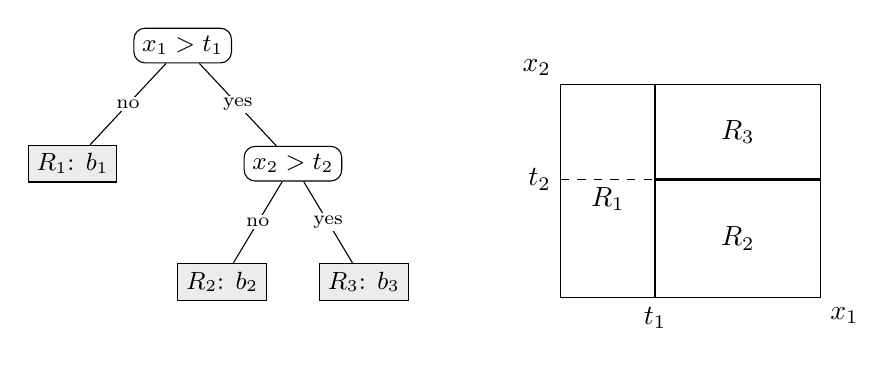
\begin{tikzpicture}[
      split/.style={draw, rounded corners, inner sep=3pt, font=\small},
      leaf/.style={draw, fill=gray!15, inner sep=3pt, font=\small},
      lbl/.style={font=\scriptsize, fill=white, inner sep=1pt}]
      % tree
      \node[split] (root) at (0, 0)      {$x_1 > t_1$};
      \node[leaf]  (r1)   at (-1.4, -1.5) {$R_1$: $b_1$};
      \node[split] (n2)   at (1.4, -1.5)  {$x_2 > t_2$};
      \node[leaf]  (r2)   at (0.5, -3)    {$R_2$: $b_2$};
      \node[leaf]  (r3)   at (2.3, -3)    {$R_3$: $b_3$};
      \draw (root) -- node[lbl] {no}  (r1);
      \draw (root) -- node[lbl] {yes} (n2);
      \draw (n2)   -- node[lbl] {no}  (r2);
      \draw (n2)   -- node[lbl] {yes} (r3);
      % induced partition of the feature space
      \begin{scope}[xshift=4.8cm, yshift=-3.2cm]
        \draw (0, 0) rectangle (3.3, 2.7);
        \draw[thick] (1.2, 0) -- (1.2, 2.7);
        \draw[thick] (1.2, 1.5) -- (3.3, 1.5);
        \draw[dashed] (0, 1.5) -- (1.2, 1.5);
        \node at (0.6, 1.25)  {$R_1$};
        \node at (2.25, 0.75) {$R_2$};
        \node at (2.25, 2.1)  {$R_3$};
        \node[below]       at (1.2, 0)   {$t_1$};
        \node[left]        at (0, 1.5)   {$t_2$};
        \node[below right] at (3.3, 0)   {$x_1$};
        \node[above left]  at (0, 2.7)   {$x_2$};
      \end{scope}
    \end{tikzpicture}
    \caption{A regression tree of depth two on two features (left) and the
    partition of the feature space it induces (right). Each leaf corresponds to a
    rectangular region $R_j$ and returns the constant $b_j$.}
    \label{fig:bg:gbm:tree}
    \end{figure}
    
    Once the regions are fixed, the leaf values follow directly: each $b_j$ is the
    constant that minimizes the loss over the training examples falling in $R_j$.
    Under squared error this is the mean of their targets, while a classification
    tree predicts the most frequent class in the leaf, or the class frequencies
    when probabilities are needed~\cite{hastie2009}. Choosing the regions is the
    hard part. Finding the partition with the lowest total loss is computationally
    infeasible in general, so trees are grown greedily from the top: at each node
    every feature and every candidate threshold is tried, and the split that most
    reduces the training loss is kept. Growth goes on
    until a stopping rule is met, such as a maximum depth or a minimum number of
    examples per leaf.

    Depth is the main control on a tree's complexity, since a tree of depth $d$ has
    at most $2^d$ leaves. A shallow tree has too few regions to follow a complex
    relation between features and target, and underfits; a deep tree can
    isolate small groups of training examples and overfits the training set.
    Trees are also unstable. Every split depends on the ones above it, so an
    error near the root propagates to the whole subtree below, and a small
    change in the training data can produce a very different tree. Ensembles of
    many trees, built by bagging or by boosting, mitigate both problems.

    \subsection{Bagging and Boosting}
    \label{subsec:bg:gbm:boosting}
    The simplest way to combine trees is \emph{bagging}, a name that stands for
    \emph{bootstrap aggregating}~\cite{breiman1996}. From the training set
    $\mathcal{D}$ one draws $B$ bootstrap samples, each of size $N$, by picking
    examples uniformly at random with replacement. The same learning algorithm is
    trained independently on each sample, which gives $B$ models
    $h_1, \dots, h_B$, and their predictions are merged at the end. For regression
    they are averaged,
    \begin{equation}
    F(x) = \frac{1}{B} \sum_{b=1}^{B} h_b(x),
    \label{eq:bg:gbm:bagging}
    \end{equation}
    and for classification the predicted class is decided by majority
    vote.
    
    Bagging works by reducing variance. Since the bootstrap samples differ, an
    unstable learner such as a deep tree fits different noise on each of them and
    makes different errors, which partly cancel out in the average. How much they
    cancel depends on how correlated the models are. If the $B$ predictions at a
    point $x$ share the same variance $\sigma^2$ and have pairwise correlation
    $\rho$, their average has variance~\cite{hastie2009}
    \begin{equation}
    \rho\, \sigma^{2} + \frac{1 - \rho}{B}\, \sigma^{2}.
    \label{eq:bg:gbm:bagvar}
    \end{equation}
    For independent models ($\rho = 0$) this is $\sigma^2 / B$, which vanishes as
    $B$ grows. Bootstrap samples, however, all come from the same dataset, so the
    models stay correlated, and the first term sets a floor that adding more
    models cannot lower. Random forests~\cite{breiman2001} push the correlation
    down further by also restricting each split to a random subset of the
    features. The bias does not improve: the models are identically distributed,
    so the expected value of their average equals that of any single one of
    them. Bagging therefore pays off with learners of low bias
    and high variance, such as deep trees, and brings little to simple, stable
    ones.
    
    \emph{Boosting} builds the models in sequence. Each new model is trained on
    a version of the data that emphasizes the examples the models built so far
    handle badly, and the final prediction is a weighted combination of all of
    them, in which the better models count more. Since every model corrects
    systematic errors of the ensemble built before it, boosting reduces bias as
    well as variance, and it works even with trees that have a single split
    (\emph{stumps}), which have low variance and high bias and gain almost nothing
    from bagging~\cite{friedman2000}.
    
    The idea grew out of a question in learning theory. Kearns and
    Valiant~\cite{kearns1994} distinguished a \emph{strong} learner, which with
    high probability reaches an arbitrarily small error, from a \emph{weak}
    learner, which only has to do slightly better than random guessing on any
    distribution of the examples, and asked whether a weak learner can always be
    turned into a strong one. Schapire~\cite{schapire1990} proved that it can,
    with a construction that retrains the weak learner on filtered versions of the
    data focused on the examples the previous hypotheses got wrong and combines
    the resulting hypotheses by majority vote, and Freund~\cite{freund1995} later
    made the scheme more efficient. Both algorithms had to know in advance by how
    much the weak learner beats chance. AdaBoost~\cite{freund1997} dropped that
    requirement: after every round it reweights the training examples according to
    the error of the latest weak learner, and it weights each learner in the final
    vote by its accuracy.
    
    Friedman, Hastie and Tibshirani~\cite{friedman2000} later explained what
    AdaBoost does in statistical terms. It builds an additive model
    $F(x) = \sum_{m=1}^{M} \alpha_m h_m(x)$ one term at a time, and each round is a
    step that minimizes the exponential loss $\mathbb{E}\bigl[e^{-y F(x)}\bigr]$,
    with labels $y \in \{-1, +1\}$. Seen this way, boosting is a numerical
    optimization procedure, and nothing forces the loss to be the exponential one.

    \subsection{Gradient Boosting}
    \label{subsec:bg:gbm:gradient}
    Gradient boosting generalizes this view to any differentiable loss. It
    builds an additive model by gradient descent, adding one base learner at each
    iteration~\cite{friedman2001}. The model is a sequence of approximations
    $F^{(0)}, F^{(1)}, \dots$, each obtained from the previous one as
    \begin{equation}
    F^{(t)}(x) = F^{(t-1)}(x) + \eta^{(t)} h^{(t)}(x),
    \label{eq:bg:gbm:stagewise}
    \end{equation}
    where $\eta^{(t)}$ is a step size and the base learner $h^{(t)}$ is taken from
    a family $\mathcal{H}$ of simple functions, such as trees of bounded depth, so
    as to reduce the expected loss~\eqref{eq:bg:gbm:exploss} as much as possible:
    \begin{equation}
    h^{(t)}
    = \arg\min_{h \in \mathcal{H}} \mathcal{L}\bigl(F^{(t-1)} + h\bigr)
    = \arg\min_{h \in \mathcal{H}}
      \mathbb{E}\bigl[ L\bigl(y, F^{(t-1)}(x) + h(x)\bigr) \bigr].
    \label{eq:bg:gbm:hstep}
    \end{equation}
    For most losses and base learners \eqref{eq:bg:gbm:hstep} cannot be solved
    exactly, and it is approximated either by a gradient step or by a Newton
    step~\cite{prokhorenkova2018}.
    
    The gradient step comes from steepest descent, which minimizes a function of
    a parameter vector by moving the vector, at each iteration, in the direction
    of the negative gradient. Gradient boosting applies the same rule in
    function space, treating the value $F(x)$ at each point $x$ as a parameter
    in its own right. The
    gradient of the loss with respect to that value, at the current model, is
    \begin{equation}
    g^{(t)}(x, y) =
    \frac{\partial L(y, s)}{\partial s} \bigg|_{s = F^{(t-1)}(x)},
    \label{eq:bg:gbm:grad}
    \end{equation}
    and $-g^{(t)}(x, y)$ is the direction in which the loss decreases fastest. On a
    finite dataset this gradient is defined only at the $N$ training points and
    says nothing about new inputs, so gradient boosting projects
    it onto $\mathcal{H}$. It computes the pseudo-residuals
    $r_i^{(t)} = -g^{(t)}(x^{(i)}, y^{(i)})$ and fits the base learner to them by
    least squares,
    \begin{equation}
    h^{(t)} = \arg\min_{h \in \mathcal{H}}
    \sum_{i=1}^{N} \bigl( r_i^{(t)} - h(x^{(i)}) \bigr)^{2},
    \label{eq:bg:gbm:lsfit}
    \end{equation}
    which selects the member of $\mathcal{H}$ most parallel to the negative
    gradient. The original loss comes back
    only in the choice of the step, through a one-dimensional \emph{line search}:
    \begin{equation}
    \eta^{(t)} = \arg\min_{\eta}
    \sum_{i=1}^{N} L\bigl( y^{(i)}, F^{(t-1)}(x^{(i)}) + \eta\, h^{(t)}(x^{(i)}) \bigr).
    \label{eq:bg:gbm:linesearch}
    \end{equation}
    Any differentiable loss can thus be minimized with nothing more than a
    least-squares fitting routine for the base learner.

    The Newton step also uses second-order information. Newton's method minimizes
    a function by replacing it, at every iteration, with its second-order Taylor
    approximation around the current point and jumping to the minimum of that
    quadratic; for a scalar function $\ell(s)$ the update is
    $s \leftarrow s - \ell'(s) / \ell''(s)$. In gradient boosting the expansion is
    taken around the current model,
    \begin{equation}
    L\bigl(y, F^{(t-1)}(x) + h(x)\bigr) \approx
    L\bigl(y, F^{(t-1)}(x)\bigr) + g^{(t)}(x, y)\, h(x)
    + \tfrac{1}{2}\, \kappa^{(t)}(x, y)\, h(x)^{2},
    \label{eq:bg:gbm:taylor}
    \end{equation}
    where $\kappa^{(t)}(x, y)$ is the second derivative of $L(y, s)$ with respect
    to $s$ at $s = F^{(t-1)}(x)$. Minimizing the right-hand side point by point
    gives the step $-g^{(t)} / \kappa^{(t)}$, and the base learner is fitted to
    these values by least squares weighted by the curvature,
    \begin{equation}
    h^{(t)} = \arg\min_{h \in \mathcal{H}}
    \sum_{i=1}^{N} \kappa_i^{(t)}
    \left( \left(-\frac{g_i^{(t)}}{\kappa_i^{(t)}}\right) - h(x^{(i)}) \right)^{2},
    \label{eq:bg:gbm:newton}
    \end{equation}
    with $g_i^{(t)}$ and $\kappa_i^{(t)}$ evaluated at the $i$-th training
    example~\cite{ibragimov2019}. The two steps coincide when the curvature is
    constant, as it is for the squared error, and differ for losses whose
    curvature changes from point to point, such as the logistic one.
    
    With the gradient step, the whole procedure is summarized in
    Algorithm~\ref{alg:bg:gbm:gb}. It starts from the best constant model and
    repeats the three operations above for $T$ iterations.
    
    \begin{algorithm}[h]
        \caption{Gradient boosting~\cite{friedman2001}}
        \label{alg:bg:gbm:gb}
        \begin{algorithmic}[1]
            \Require training set $\mathcal{D} = \{(x^{(i)}, y^{(i)})\}_{i=1}^{N}$,
                     differentiable loss $L$, base-learner family $\mathcal{H}$,
                     number of iterations $T$
            \State $F^{(0)}(x) \gets \arg\min_{c} \sum_{i=1}^{N} L\bigl(y^{(i)}, c\bigr)$
            \For{$t = 1, \dots, T$}
              \For{$i = 1, \dots, N$}
                \State $r_i^{(t)} \gets -\left.\dfrac{\partial L(y^{(i)}, s)}{\partial s}
                       \right|_{s = F^{(t-1)}(x^{(i)})}$
                       \Comment{pseudo-residuals}
              \EndFor
              \State $h^{(t)} \gets \arg\min_{h \in \mathcal{H}}
                     \sum_{i=1}^{N} \bigl( r_i^{(t)} - h(x^{(i)}) \bigr)^{2}$
                     \Comment{least-squares fit}
              \State $\eta^{(t)} \gets \arg\min_{\eta} \sum_{i=1}^{N}
                     L\bigl( y^{(i)}, F^{(t-1)}(x^{(i)}) + \eta\, h^{(t)}(x^{(i)}) \bigr)$
                     \Comment{line search}
              \State $F^{(t)}(x) \gets F^{(t-1)}(x) + \eta^{(t)} h^{(t)}(x)$
            \EndFor
            \State \Return $F^{(T)}$
        \end{algorithmic}
    \end{algorithm}
    When the base learners are regression trees \eqref{eq:bg:gbm:tree}, the update
    becomes
    \begin{equation}
    F^{(t)}(x) = F^{(t-1)}(x) + \eta^{(t)} \sum_{j=1}^{J} b_j^{(t)}\,
    \mathbb{I}{\{x \in R_j^{(t)}\}},
    \end{equation}
    where the regions $R_j^{(t)}$ are the leaves of the tree grown on the
    pseudo-residuals and $b_j^{(t)}$ is the constant the tree predicts in leaf
    $j$. Because the leaves are disjoint, the least-squares fit
    \eqref{eq:bg:gbm:lsfit} splits into one independent problem per leaf,
    \begin{equation}
        b_j^{(t)} = \arg\min_{b} \sum_{x^{(i)} \in R_j^{(t)}} \bigl( r_i^{(t)} - b \bigr)^{2}
        = \frac{1}{N_j^{(t)}} \sum_{x^{(i)} \in R_j^{(t)}} r_i^{(t)},
        \label{eq:bg:gbm:leafmean}
    \end{equation}
    where $N_j^{(t)}$ is the number of training examples in the leaf. Each
    $b_j^{(t)}$ is therefore the mean pseudo-residual of the examples that fall in
    leaf $j$. The same disjointness means the tree can also be read
    as $J$ separate basis functions, one per leaf, each of which may receive its
    own coefficient. Friedman therefore replaces the single line search with a
    separate one in every leaf~\cite{friedman2001},
    \begin{equation}
    \eta_j^{(t)} = \arg\min_{\eta}
    \sum_{x^{(i)} \in R_j^{(t)}} L\bigl( y^{(i)}, F^{(t-1)}(x^{(i)}) + \eta \bigr),
    \qquad
    F^{(t)}(x) = F^{(t-1)}(x) + \sum_{j=1}^{J} \eta_j^{(t)}\,
    \mathbb{I}{\{x \in R_j^{(t)}\}}.
    \label{eq:bg:gbm:leaf}
    \end{equation}
    The structure of the tree is learned from the gradient by least squares, while
    the leaf values are fitted on the original loss. When the minimization in
    \eqref{eq:bg:gbm:leaf} has no closed form, it is approximated by one or a
    few Newton steps; a single step gives, in leaf $j$,
    $\eta_j^{(t)} = -\sum_{x^{(i)} \in R_j^{(t)}} g_i^{(t)} \big/
    \sum_{x^{(i)} \in R_j^{(t)}} \kappa_i^{(t)}$.
    
    For regression the usual loss is the squared error,
    \begin{equation}
    L(y, F) = \tfrac{1}{2}\,(y - F)^{2},
    \label{eq:bg:gbm:mse}
    \end{equation}
    whose average over the data is the mean squared error. Its square root, the
    root mean squared error (RMSE), is a monotone function of it, so minimizing
    either one gives the same model. Here $g^{(t)} = F^{(t-1)}(x) - y$ and
    $\kappa^{(t)} = 1$: the pseudo-residuals are the ordinary residuals
    $y - F^{(t-1)}(x)$, the gradient and Newton steps coincide, and the optimal
    value of each leaf is the mean residual of its examples.
    
    For binary classification with labels $y \in \{0, 1\}$, $F(x)$ is read as the
    log-odds of the positive class, so that
    $p(x) = 1 / \bigl(1 + e^{-F(x)}\bigr)$, and the loss is the negative
    log-likelihood of a Bernoulli variable, known as the \emph{logarithmic loss}:
    \begin{equation}
    L(y, F) = -\bigl[\, y \ln p(x) + (1 - y) \ln\bigl(1 - p(x)\bigr) \bigr].
    \label{eq:bg:gbm:logloss}
    \end{equation}
    Its derivatives with respect to $F$ are $g^{(t)} = p(x) - y$ and
    $\kappa^{(t)} = p(x)\bigl(1 - p(x)\bigr)$, with $p$ computed from
    $F^{(t-1)}$. The pseudo-residuals $y - p(x)$ are therefore residuals on the
    probability scale, and the Newton value of leaf $j$ is
    \begin{equation}
    \eta_j^{(t)} =
    \frac{\sum_{x^{(i)} \in R_j^{(t)}} \bigl( y^{(i)} - p(x^{(i)}) \bigr)}
         {\sum_{x^{(i)} \in R_j^{(t)}} p(x^{(i)}) \bigl( 1 - p(x^{(i)}) \bigr)}.
    \label{eq:bg:gbm:loglossleaf}
    \end{equation}
    Friedman~\cite{friedman2001} and Friedman, Hastie and
    Tibshirani~\cite{friedman2000} write the same algorithm with labels in
    $\{-1, +1\}$ and $F$ equal to half the log-odds, which changes the constants
    but not the procedure.
    
    Left unchecked, the procedure keeps lowering the training loss and
    eventually overfits. The number of iterations $T$ is the most direct control,
    since every tree adds capacity, but regularization through \emph{shrinkage}
    has often been found to work better than limiting the number of
    terms. Each update is scaled by a \emph{learning rate}
    $0 < \epsilon \le 1$,
    \begin{equation}
    F^{(t)}(x) = F^{(t-1)}(x) + \epsilon\, \eta^{(t)} h^{(t)}(x),
    \label{eq:bg:gbm:shrinkage}
    \end{equation}
    so that the model moves only part of the way along each step. The two
    parameters trade off against each other. A smaller $\epsilon$ needs more trees
    to reach the same training loss, but in Friedman's experiments it also gave a
    lower error on held-out data and much less overfitting as trees were added,
    with diminishing returns for the smallest values~\cite{friedman2001}. In
    practice $\epsilon$ is set small and $T$ is chosen by monitoring the loss on
    data left out of training while trees are added. Stopping
    as soon as that held-out loss stops improving is known as \emph{early
    stopping}, and it also avoids training trees that would only hurt the model.
    
    The size of each tree is the other control on capacity. A tree with $J$ leaves
    can model interactions among at most $\min(J - 1, m)$ features, and a tree of
    depth $d$ among at most $d$, since no path from the root to a leaf tests more
    than $d$ features. Stumps therefore give a model that is additive in the
    individual features, and deeper trees allow interactions of higher order. The
    best size depends on the interaction order of the function being learned, and
    since the targets met in practice are often well approximated by low-order
    interactions, large trees are rarely needed.
    
    \emph{Stochastic gradient boosting}~\cite{friedman2002} adds randomness to the
    procedure: at every iteration the tree is fitted on a random subsample of the
    training set, drawn uniformly without replacement, rather than on all of it.
    Each tree becomes cheaper to build, roughly in proportion to the sampling
    rate, and in many cases the ensemble also generalizes better. Subsampling makes
    each tree noisier, but it lowers the correlation between trees, the same
    quantity that limits the variance reduction of bagging
    in~\eqref{eq:bg:gbm:bagvar}~\cite{ibragimov2019}.

    \subsection{CatBoost}
    \label{subsec:bg:gbm:catboost}
    CatBoost~\cite{prokhorenkova2018,dorogush2018} is an open-source
    implementation of gradient boosting with decision trees. Its authors observed
    that, in the procedure of Section~\ref{subsec:bg:gbm:gradient}, the gradients
    of each iteration are computed on the same examples that were used to build
    the current model, which fits those examples better than it would fit new
    ones. The trees are then learned from slightly biased gradients, an effect
    they call \emph{prediction shift}. To avoid it, CatBoost offers an
    \emph{Ordered} boosting mode, in which the gradient of each example comes
    from a model trained only on the examples that precede it in a random
    permutation of the training set, and uses the same idea to encode
    categorical features. The bias shrinks as the training set grows, and in the
    authors' experiments the Ordered mode gave its largest gains below about
    40{,}000 training examples. Next to it CatBoost keeps a \emph{Plain} mode,
    which follows the standard procedure: the structure of each tree is chosen
    from the gradients, and once the splits are fixed the leaf values are
    computed with the Newton step of Section~\ref{subsec:bg:gbm:gradient}.

    Whichever mode is used, the trees themselves differ from those of
    Section~\ref{subsec:bg:gbm:trees}. CatBoost builds \emph{oblivious} trees,
    also called decision tables, in which the same split is used for every node of
    a level. A tree of depth $d$ is then
    just a list of $d$ conditions $x_{k_\ell} > t_\ell$, $\ell = 1, \dots, d$, and
    the index of the leaf reached by $x$ is read off the binary number formed by
    their outcomes,
    \begin{equation}
    j(x) = 1 + \sum_{\ell=1}^{d} 2^{\ell - 1}\, \mathbb{I}\{x_{k_\ell} > t_\ell\},
    \qquad j(x) \in \{1, \dots, 2^{d}\},
    \label{eq:bg:gbm:oblivious}
    \end{equation}
    so that $x$ falls in the region $R_{j(x)}$ of~\eqref{eq:bg:gbm:tree}, now with
    $J = 2^d$ leaves. Oblivious trees are balanced and, being so constrained,
    less prone to overfitting than unrestricted trees of the same depth;
    prediction reduces to $d$ comparisons and a table lookup, which makes it very
    fast. As an alternative, CatBoost can
    grow ordinary trees level by level, splitting every node of the last level
    with its own best condition until the maximum depth is reached (the
    \emph{Depthwise} policy). A minimum number of training examples per leaf can
    then be imposed, and no split is searched in a leaf with fewer
    examples~\cite{catboostdocs}.

    The logarithmic loss and the squared error of
    Section~\ref{subsec:bg:gbm:gradient} are available in CatBoost as
    \texttt{Logloss} and \texttt{RMSE}, together with \texttt{RMSEWithUncertainty},
    which makes the model predict the mean and the variance of a Normal
    distribution and minimizes its negative log-likelihood~\cite{malinin2021}.

    CatBoost also randomizes the examples that each tree sees, as
    stochastic gradient boosting does, and offers three ways of doing it. The
    \emph{Bayesian bootstrap} removes no example. At every iteration each example
    receives a random weight $w_i$, which multiplies its gradient when the tree
    structure is chosen~\cite{rubin1981},
    \begin{equation}
    w_i = \bigl( -\log \psi_i \bigr)^{\omega},
    \qquad \psi_i \sim \mathcal{U}(0, 1),
    \label{eq:bg:gbm:bayesboot}
    \end{equation}
    where the \emph{bagging temperature} $\omega \ge 0$ controls how uneven the
    weights are~\cite{catboostdocs}. \emph{Bernoulli} sampling, instead,
    removes examples. At every iteration each example is kept with probability
    $q$, the sampling rate, and discarded otherwise, independently of the others,
    and the splits of the new tree are chosen using only the examples that were
    kept, on average a fraction $q$ of the training
    set~\cite{catboostbootstrap}.

    Both schemes treat all examples alike, and \emph{minimal variance sampling}
    (MVS)~\cite{ibragimov2019} drops that assumption. Its starting observation is
    that a subsample only serves to estimate the scores of candidate splits, which
    are built from the sums of gradients and curvatures in each leaf. MVS
    therefore chooses the sampling probabilities that minimize the variance of
    these estimates for an expected subsample size of $qN$. Up to an
    approximation of the score, the solution is
    \begin{equation}
    p_i = \min\Biggl( 1,\;
    \frac{\sqrt{\bigl(g_i^{(t)}\bigr)^2 + \delta \bigl(\kappa_i^{(t)}\bigr)^2}}{\vartheta} \Biggr),
    \qquad \sum_{i=1}^{N} p_i = qN,
    \label{eq:bg:gbm:mvs}
    \end{equation}
    where the threshold $\vartheta$ is set so that the constraint holds and
    $\delta \ge 0$ is a regularization coefficient. Examples
    whose regularized gradient exceeds $\vartheta$, those the current model fits
    worst, are always kept, and the others are kept with a probability
    proportional to it. Each sampled example then receives the weight $1/p_i$,
    which keeps the sums of gradients and curvatures in each leaf unbiased. The
    coefficient $\delta$ moves the scheme between two known cases: as $\delta \to
    0$ it becomes importance sampling on the gradients, and with first-order
    steps, where $\kappa_i^{(t)} = 1$ for every example, as $\delta \to \infty$
    all probabilities become equal and it falls back to uniform sampling.

    Features can be sampled as well as examples. With the random subspace method,
    each time a split is selected only a random fraction of the features is
    considered~\cite{catboostdocs}, which adds randomness to the trees in the same
    way that sampling the examples does.

    The leaf values, finally, are regularized directly, by adding to the training
    loss an L2 penalty on them~\cite{chen2016}:
    \begin{equation}
    \sum_{i=1}^{N} L\bigl(y^{(i)}, F(x^{(i)})\bigr)
    + \tfrac{1}{2}\, \zeta \sum_{j} \eta_j^{2},
    \label{eq:bg:gbm:l2loss}
    \end{equation}
    where $\zeta \ge 0$ is the regularization coefficient. Large leaf values now
    have a cost, so the model prefers smaller ones. Minimizing the second-order
    expansion of~\eqref{eq:bg:gbm:l2loss} instead of the plain loss adds $\zeta$
    to the denominator of the Newton leaf value of
    Section~\ref{subsec:bg:gbm:gradient},
    \begin{equation}
    \eta_j^{(t)} =
    -\frac{\sum_{x^{(i)} \in R_j^{(t)}} g_i^{(t)}}
        {\sum_{x^{(i)} \in R_j^{(t)}} \kappa_i^{(t)}}
    \quad \longrightarrow \quad
    \eta_j^{(t)} =
    -\frac{\sum_{x^{(i)} \in R_j^{(t)}} g_i^{(t)}}
        {\sum_{x^{(i)} \in R_j^{(t)}} \kappa_i^{(t)} + \zeta}.
    \label{eq:bg:gbm:l2leaf}
    \end{equation}
    For the squared error, where $\kappa_i^{(t)} = 1$, the denominator becomes the
    number of examples in the leaf plus $\zeta$. A leaf estimated from a handful
    of examples is then pulled strongly toward zero, while one estimated from
    thousands barely changes.

% #############################################################################

\section{Predictive Uncertainty Quantification}
\label{sec:bg:uncertainty}
A trained model turns an input into a prediction, and on its own that
prediction is just a value with no indication of how far it can be trusted.
For many uses this is fine. When a wrong prediction is costly, the model is
expected to also report how confident it is, so that uncertain cases can be
flagged and handed to a human or to a safe default rather than acted on
blindly~\cite{malinin2021}. Why a prediction may be wrong matters as well:
the data may be inherently noisy, or the model may be extrapolating to inputs
it has rarely seen, and the two call for different responses.

\subsection{Aleatoric and Epistemic Uncertainty}
    \label{subsec:bg:uncertainty:taxonomy}
    The sources of uncertainty are usually defined in a Bayesian
    setting~\cite{malinin2021}. Let a
    model be described by parameters $\theta$ and trained on a dataset
    $\mathcal{D} = \{(x^{(i)}, y^{(i)})\}_{i=1}^{N}$. Treating $\theta$ as a random
    variable with a prior $p(\theta)$, Bayes' rule gives the posterior
    \begin{equation}
        p(\theta \mid \mathcal{D}) =
        \frac{p(\mathcal{D} \mid \theta)\, p(\theta)}{p(\mathcal{D})}.
        \label{eq:bg:unc:bayes}
    \end{equation}
    Each value of $\theta$ is one hypothesis about how the data is generated, and
    the posterior concentrates on the hypotheses that agree with what has been
    observed. A prediction for a new input $x$ averages over them,
    \begin{equation}
        P(y \mid x, \mathcal{D}) =
        \mathbb{E}_{p(\theta \mid \mathcal{D})}\!\left[\, P(y \mid x; \theta) \,\right],
        \label{eq:bg:unc:predpost}
    \end{equation}
    and the quantity to characterize is the spread of this predictive
    distribution, measured by its entropy
    \begin{equation}
        \mathcal{H}\!\left[ P(y \mid x, \mathcal{D}) \right] = \mathbb{E}_{P(y \mid x, \mathcal{D})}\!\left[ -\ln P(y \mid x, \mathcal{D}) \right].
    \end{equation}
    The spread has two sources, which behave differently:
    \begin{itemize}
        \item \emph{Aleatoric} uncertainty, also called \emph{data} uncertainty, is the irreducible noise of the process itself: label noise, overlapping classes, features that do not determine the target. It is a property of the data rather than of the model, so more training examples do not reduce it; it may be constant over the input space (homoscedastic) or depend on $x$ (heteroscedastic). 
        
        \item \emph{Epistemic} uncertainty, also called \emph{knowledge} or \emph{model} uncertainty, is the model's lack of knowledge. It is large where training data is sparse or absent, because there the posterior still spreads over many values of $\theta$ that extrapolate in different ways, and it is small where the data is dense and those values agree. It shrinks as the training set grows, and it is the component that rises on inputs drawn from outside the training distribution.
    \end{itemize}
    Aleatoric uncertainty sets how wide an honest prediction interval has to be
    even for an ideal model. Epistemic uncertainty signals when the model is
    extrapolating, so that its output should be discounted regardless of how
    narrow that interval looks~\cite{gal2016,hullermeier2021}.
    \begin{figure}[h]
      \centering
      \includegraphics[width=0.8\linewidth]{chapters/2_Background/2_images/aleatoric_epistemic.pdf}
      \caption{Aleatoric and epistemic uncertainty on a one-dimensional regression
        problem. Training data is available in two regions, tightly and with little
        noise on the left, sparsely and with heavy noise on the right, and absent
        in between and outside the range. The orange band is the data (aleatoric)
        uncertainty: it tracks the local noise level, wide on the right and narrow
        on the left, and does not shrink with more data. The blue band is the total
        predictive uncertainty; where it exceeds the orange band the model is
        extrapolating, and the excess is the knowledge (epistemic) uncertainty,
        which collapses to zero wherever the data is dense.}
      \label{fig:bg:unc:types}
    \end{figure}

\subsection{Decomposing Uncertainty with Ensembles}
    \label{subsec:bg:uncertainty:ensembles}
    \label{subsec:bg:uncertainty:stats}
    A single model cannot separate the two sources, because one value of
    $\theta$ cannot disagree with itself; an ensemble can. Take $M$ parameter
    vectors $\{\theta^{(m)}\}_{m=1}^{M}$ drawn approximately from the posterior
    $p(\theta \mid \mathcal{D})$. The predictive distribution
    \eqref{eq:bg:unc:predpost} is approximated by the average over the members,
    \begin{equation}
        P(y \mid x, \mathcal{D}) \approx \frac{1}{M} \sum_{m=1}^{M} P(y \mid x; \theta^{(m)}),
        \label{eq:bg:unc:ensavg}
    \end{equation}
    so that the total uncertainty is the entropy of this average, while the two
    components are recovered by comparing the average against the members taken
    one at a time.

    \subsubsection{Classification}  
        Let $\mathcal{H}[p] = -\sum_k p_k \ln p_k$ be the Shannon entropy of a
        distribution $p$ over the labels and $\mathcal{I}[\,\cdot\,,\cdot\,]$
        the mutual information between two random variables. The decomposition is
        then exact~\cite{malinin2021,depeweg2017decomposition,depeweg2018}:
        \begin{align}
            \underbrace{\mathcal{I}\!\left[ y, \theta \mid x, \mathcal{D} \right]}_{\text{Knowledge Uncertainty}} 
            &= \underbrace{\mathcal{H}\!\left[ P(y \mid x, \mathcal{D}) \right]}_{\text{Total Uncertainty}} - \underbrace{\mathbb{E}_{p(\theta \mid \mathcal{D})}\!\left[\, \mathcal{H}\!\left[ P(y \mid x,\theta) \right]\right]}_{\text{Data Uncertainty}} \\[1.2ex]
            &\approx 
            \underbrace{\mathcal{H}\!\left[ \frac{1}{M} \sum_{m=1}^{M} P(y \mid x; \theta^{(m)}) \right]}_{\text{Total Uncertainty}} - \underbrace{\frac{1}{M} \sum_{m=1}^{M} \mathcal{H}\!\left[ P(y \mid x; \theta^{(m)}) \right]}_{\text{Data Uncertainty}}
        \end{align}
        Total uncertainty is the entropy of the averaged prediction. The data term is
        the mean entropy of the individual members, that is, the uncertainty left once
        the model is fixed. Their difference is the mutual information between the
        parameters and the label: it is exactly the disagreement among the members,
        and vanishes when they all predict the same distribution.

    \subsubsection{Regression}
        The differential entropy of the averaged distribution has no closed form, so
        the same split is applied to the variance, through the law of total
        variance~\cite{malinin2021}:
        \begin{equation}
            \underbrace{\operatorname{Var}_{p(y \mid x, \mathcal{D})}[y]}_{\text{Total Uncertainty}}
            =
            \underbrace{\operatorname{Var}_{p(\theta \mid \mathcal{D})}\!\bigl[ \mathbb{E}_{p(y \mid x, \theta)}[y] \bigr]}_{\text{Knowledge Uncertainty}}
            +
            \underbrace{\mathbb{E}_{p(\theta \mid \mathcal{D})}\!\bigl[ \operatorname{Var}_{p(y \mid x,\theta)}[y] \bigr]}_{\text{Data Uncertainty}} .
            \label{eq:bg:unc:totvar}
        \end{equation}
        This needs each member to report a variance, not just a point value. A
        gradient-boosted regressor trained under squared error does not; the standard
        fix, introduced with NGBoost~\cite{duan2020ngboost} and adopted by Malinin et
        al.~\cite{malinin2021}, is to let the model predict the mean and the log
        standard deviation $\bigl(\mu(x), \log \sigma(x)\bigr)$ of a Normal
        distribution and to train it by minimizing the negative log-likelihood. With
        member $m$ then reporting a mean $\mu_m$ and a variance $\sigma_m^2$, and
        $\bar\mu = \tfrac{1}{M}\sum_m \mu_m$, the two terms of the total variance
        become
        \begin{equation}
            \underbrace{\operatorname{Var}_{p(y \mid x,\mathcal{D})}[y]}_{\text{Total Uncertainty}} \approx
            \underbrace{\frac{1}{M} \sum_{m=1}^{M} (\mu_m - \bar\mu)^2}_{\text{Knowledge Uncertainty}}
            +
            \underbrace{\frac{1}{M} \sum_{m=1}^{M} \sigma_m^2}_{\text{Data Uncertainty}} .
            \label{eq:bg:unc:gaussvar}
        \end{equation}
        Knowledge uncertainty is the variance of the predicted means, data uncertainty
        is the mean of the predicted variances, and the total predictive standard
        deviation is the square root of their sum. Both estimators use only the first
        two moments of the member distributions, so they can miss higher-order
        structure of the predictive distribution, and neither is
        scale-invariant~\cite{malinin2021}.

\subsection{Uncertainty in Gradient-Boosted Decision Trees}
    \label{subsec:bg:uncertainty:gbm}
    The ensemble decomposition needs parameter samples $\{\theta^{(m)}\}$,
    whereas a boosted model is a deterministic sequence of trees. Malinin et
    al.~\cite{malinin2021} describe three ways to obtain them: perturb the
    training with extra randomness, turn the training itself into a sampler of
    the posterior, or reuse the intermediate stages of a single model.

    \subsubsection{Stochastic gradient boosting} 
        Stochastic gradient boosting takes the first route. Several models are
        trained independently, each with its own seed for the row subsampling the
        algorithm already performs~\cite{friedman2002}, and the subsampling perturbs
        every fit enough to spread the learned parameters out. The spread,
        however, is uncontrolled: nothing ties it to the posterior $p(\theta \mid \mathcal{D})$, so
        the disagreement among the models has no formal reading as epistemic
        uncertainty.
    
    \subsubsection{Stochastic gradient Langevin boosting} 
        Stochastic gradient Langevin boosting (SGLB) closes that gap by making the training a posterior sampler. It adds Gaussian noise to the gradient at every iteration,
        \begin{equation}
        h^{(t)} = \arg\min_{h \in \mathcal{H}}
        \mathbb{E}_{\mathcal{D}}\!\left[ \bigl( -g^{(t)}(x, y) - h(x, \phi) + \nu \bigr)^{2} \right],
        \qquad
        \nu \sim \mathcal{N}\!\left( 0, \tfrac{2}{\beta \epsilon}\, I_{|\mathcal{D}|} \right),
        \label{eq:bg:unc:sglbnoise}
        \end{equation}
        and replaces the plain additive update with a shrinking one,
        \begin{equation}
        F^{(t)}(x) = (1 - \gamma \epsilon)\, F^{(t-1)}(x) + \epsilon\, h^{(t)}(x, \phi^{(t)}),
        \label{eq:bg:unc:sglbupdate}
        \end{equation}
        where $\phi$ denotes the parameters of a tree, $\epsilon$ is the
        learning rate, $\gamma$ a shrinkage coefficient and $\beta$ the inverse
        of the diffusion temperature. Under these dynamics the parameter sequence $\theta^{(t)}$ is a Markov chain
        that converges weakly to the stationary distribution
        $p^{*}_{\beta}(\theta) \propto
        \exp\!\bigl( -\beta\, \mathcal{L}(\theta \mid \mathcal{D})
        - \beta \gamma \lVert \Gamma \theta \rVert_2^2 \bigr)$,
        with $\Gamma$ an implicitly defined regularization matrix. Setting
        $\beta = \lvert \mathcal{D} \rvert$ and $\gamma = 1 / (2\lvert \mathcal{D} \rvert)$
        makes that stationary distribution proportional to
        $p(\mathcal{D} \mid \theta)\, p(\theta)$ under a Gaussian prior $p(\theta) = \mathcal{N}(0,\Gamma)$, that is, to
        the true posterior~\cite{ustimenko2021sglb}. A single SGLB run therefore
        produces, in its later iterations, a trajectory of approximate posterior
        samples, with no need to train several models.
    
    \subsubsection{Virtual ensembles} 
        Virtual ensembles turn that trajectory into ensemble members at no
        extra training cost. A boosted model of $T$ trees is a sum of weak learners,
        so its truncations to the first $t$ trees are themselves models and can serve
        as members. To keep them from being near-duplicates, only every $K$-th
        truncation is kept, and only from the second half of the run, where the chain
        has reached its stationary regime:
        \begin{equation}
        \Theta_{T,K} =
        \Bigl\{ \theta^{(Kt)} \;:\;
        \bigl\lceil \tfrac{T}{2K} \bigr\rceil \le t \le \bigl\lfloor \tfrac{T}{K} \bigr\rfloor
        \Bigr\}.
        \label{eq:bg:unc:virtual}
        \end{equation}
        The members are read off in a single forward pass by accumulating partial
        sums of the trees, so the whole ensemble costs about as much as one model.
        They come from one correlated chain rather than from independent runs, which
        weakens the epistemic estimate relative to a true ensemble; this is the
        price of not training $M$ separate models~\cite{malinin2021}.
        \begin{figure}[h]
            \centering
            \includegraphics[width=\linewidth]{chapters/2_Background/2_images/2_virtual ensamble.png}
            \caption{Virtual ensemble: successive truncations of one boosted model act as ensemble members, each a prefix of the next, from the first few trees up to the complete model (Equation~\eqref{eq:bg:unc:virtual}).}
            \label{fig:bg:unc:virtual}
        \end{figure}


\subsection{Calibration}
    \label{subsec:bg:uncertainty:calibration}
    A model is \emph{calibrated} when its stated confidence matches its observed
    accuracy: of the cases it labels with probability $0.8$, close to $80\%$
    should turn out correct. High-capacity models tend to break this in a
    predictable direction. Once training accuracy saturates, the log-likelihood
    keeps improving by making the probabilities sharper rather than by getting
    more cases right, so the model ends up overconfident~\cite{guo2017}.
    
    \subsubsection{Classification}
        A binary classifier returns, for each case, a probability $\hat{p}$ of the
        positive class; write $\hat{P}$ for it as a random variable. The classifier
        is perfectly calibrated when that probability coincides with the frequency
        of the positive class,
        \begin{equation}
            \mathbb{P}\!\left( Y = 1 \;\middle|\; \hat{P} = p \right) = p
            \qquad \forall p \in [0, 1].
            \label{eq:bg:unc:calibclf}
        \end{equation}
        The condition cannot be checked directly: $\hat{P}$ is
        continuous, and the conditional frequency on the left cannot be estimated at a
        single value of $p$ from a finite sample~\cite{guo2017}.
        A \emph{reliability diagram} gets around this by grouping. The range $[0, 1]$ is
        cut into $Q$ equal-width bins, and $B_q$ collects the cases whose predicted
        probability falls in the $q$-th interval
        $\left( \tfrac{q-1}{Q}, \tfrac{q}{Q} \right]$. Each bin carries two numbers, the
        mean probability the model assigned and the fraction of its cases that were
        actually positive,
        \begin{equation}
            \operatorname{conf}(B_q) = \frac{1}{\lvert B_q \rvert} \sum_{i \in B_q} \hat{p}_i ,
            \qquad
            \operatorname{acc}(B_q) = \frac{1}{\lvert B_q \rvert} \sum_{i \in B_q} \mathbf{1}\{ y_i = 1 \} .
            \label{eq:bg:unc:confacc}
        \end{equation}
        The diagram plots $\operatorname{acc}(B_q)$ against $\operatorname{conf}(B_q)$,
        and a calibrated model puts every bin on the diagonal. A bin below the diagonal
        has $\operatorname{conf}(B_q) > \operatorname{acc}(B_q)$, the model claiming more
        certainty than the outcomes support, which is the direction a saturated
        classifier drifts. The vertical distance
        $\lvert \operatorname{acc}(B_q) - \operatorname{conf}(B_q) \rvert$ is the
        \emph{calibration gap} of the bin. The diagram does not show how many cases
        each bin holds, so a wide gap in a nearly empty bin looks as bad as one in a
        crowded bin.
        The \emph{expected calibration error} puts that weight back and collapses the
        diagram to one number,
        \begin{equation}
            ECE = \sum_{q=1}^{Q} \frac{\lvert B_q \rvert}{n}
            \bigl\lvert \operatorname{acc}(B_q) - \operatorname{conf}(B_q) \bigr\rvert ,
            \label{eq:bg:unc:ece}
        \end{equation}
        with $n$ the number of cases, and estimates
        $\mathbb{E}_{\hat{P}}\bigl[\, \lvert \mathbb{P}(Y = 1 \mid \hat{P} = p) - p \rvert \,\bigr]$.
        It is measured on the probability scale: an ECE of $0.05$ means that the
        probability the model assigns and the observed frequency of positives
        differ, on average over the cases, by five percentage points. Lower is
        better, and zero means a perfectly calibrated classifier.
        Its value depends on $Q$ and on the binning rule, so it is read as a
        relative measure at a fixed setting, typically compared before and after a
        calibration step~\cite{naeini2015}.

        \emph{Temperature scaling} is such a step, applied after training to the
        frozen model. The classifier forms its probability by passing a real-valued score, the
        logit $z$, through the logistic function $\sigma$, so $\hat{p} = \sigma(z)$;
        temperature scaling divides the score by a single positive constant $T$ before
        that last step,
        \begin{equation}
            \hat{p}_{\mathrm{cal}} = \sigma\!\left( z / T \right)
            = \sigma\!\bigl( \sigma^{-1}(\hat{p}) / T \bigr) .
            \label{eq:bg:unc:temp}
        \end{equation}
        At $T = 1$ nothing changes. With $T > 1$ the probability moves toward $0.5$ and
        the confidence drops; with $T < 1$ it is pushed toward the extremes. Because
        the fault being corrected is overconfidence, the fitted temperature is normally
        above one. $T$ is fitted on a held-out slice, kept apart from the data used to
        fit the model. Holding the logits $z_j$ of that slice fixed and writing
        $y_j \in \{0, 1\}$ for its labels, the temperature is the value that minimizes
        the mean log-loss of the rescaled probabilities,
        \begin{equation}
            T = \arg\min_{T > 0} \; -\frac{1}{n_{\mathrm{v}}} \sum_{j=1}^{n_{\mathrm{v}}}
            \Bigl[ y_j \ln \sigma(z_j / T)
            + (1 - y_j) \ln\bigl( 1 - \sigma(z_j / T) \bigr) \Bigr] ,
            \label{eq:bg:unc:tempfit}
        \end{equation}
        with $n_{\mathrm{v}}$ the size of the slice. This is the same log-loss used to train the
        classifier, now minimized over $T$ alone, a one-dimensional problem.
        Division by a positive constant is monotone and does not cross the $0.5$
        mark, so the predicted label and every metric computed from it stay exactly
        as they were, and only the probability attached to the label is rescaled.
        One parameter is enough because
        the overconfidence of a saturated model is close to a uniform stretch of the
        scores, which a single temperature undoes.
    
    \subsubsection{Regression}
        Calibrating a predicted distribution over a continuous target is harder, and
        the first natural definition is too weak. Following Kuleshov et
        al.~\cite{kuleshov2018}, a regression forecaster is calibrated when the target
        lands below the predicted $p$-quantile for a $p$ fraction of the data,
        \begin{equation}
            \frac{1}{n} \sum_{t=1}^{n} \mathbf{1}\!\left\{ y_t \le F_t^{-1}(p) \right\}
            \;\xrightarrow[n \to \infty]{}\; p
            \qquad \text{for all } p \in [0, 1],
            \label{eq:bg:unc:calibreg}
        \end{equation}
        where $F_t$ is the predicted cumulative distribution for example $t$. Levi et
        al.~\cite{levi2022} show that this can be satisfied by uncertainty estimates
        that carry no information: the empirical coverage is monotone in $p$, so
        fitting an isotonic regression to it produces a perfect match on the
        calibration set, and even a predicted variance drawn independently of the true
        error passes. Their alternative ties the predicted variance to the actual
        squared error, conditionally on the predicted variance itself,
        \begin{equation}
            \mathbb{E}_{x, y}\!\left[ \bigl( \mu(x) - y \bigr)^{2}
            \;\middle|\; \sigma(x)^{2} = \sigma^{2} \right] = \sigma^{2}
            \qquad \text{for all } \sigma .
            \label{eq:bg:unc:varcalib}
        \end{equation}
        Each exact value of $\sigma$ tends to occur once, so the check is again done by
        binning, this time into $Q$ groups of equal size after the examples are sorted
        by predicted standard deviation. Bin $q$ then covers a range of $\sigma$ and is
        summarized by its root mean predicted variance and its empirical root mean
        squared error,
        \begin{equation}
            \mathrm{RMV}(q) = \sqrt{ \frac{1}{\lvert B_q \rvert} \sum_{t \in B_q} \sigma_t^{2} },
            \qquad
            \mathrm{RMSE}(q) = \sqrt{ \frac{1}{\lvert B_q \rvert} \sum_{t \in B_q} (y_t - \hat{y}_t)^{2} } .
            \label{eq:bg:unc:rmvrmse}
        \end{equation}
        The first is the error size the model expects in that bin, the second the size
        it turns out to be; for a calibrated model the two agree, and the diagram that
        plots $\mathrm{RMSE}(q)$ against $\mathrm{RMV}(q)$ sits on the diagonal, just as
        the classification reliability diagram does. The scalar summary, the analogue of
        \eqref{eq:bg:unc:ece}, is the \emph{expected normalized calibration error},
        \begin{equation}
            \mathrm{ENCE} = \frac{1}{Q} \sum_{q=1}^{Q}
            \frac{\bigl\lvert \mathrm{RMV}(q) - \mathrm{RMSE}(q) \bigr\rvert}{\mathrm{RMV}(q)} .
            \label{eq:bg:unc:ence}
        \end{equation}
        Each term is a bin's gap divided by its predicted error scale, so ENCE is a
        relative error: a value of $0.1$ means that, in a typical bin, the error the
        model makes differs from the one it predicts by about $10\%$. Lower is better.
        Without that
        normalization the sum would be dominated by the high-$\sigma$ bins, where the
        errors are larger in absolute terms only because the inputs are harder. ENCE
        is zero only when the predicted and observed error sizes agree at every level
        of $\sigma$, not just on average, so a single global rescaling of $\sigma$
        need not drive it to zero.

        A low ENCE is necessary but not sufficient: a model that returns the same
        standard deviation everywhere can reach it while telling the caller nothing. It
        is read together with the \emph{coefficient of variation} of the predicted
        standard deviations,
        $c_v = \operatorname{std}(\{\sigma_t\}) / \operatorname{mean}(\{\sigma_t\})$,
        which has to sit well above zero for the uncertainty to separate one input from
        another.
        
        Recalibration is the regression counterpart of temperature scaling. Every
        predicted standard deviation is multiplied by one positive scalar $s$, fitted on
        a held-out slice by minimizing the Gaussian negative log-likelihood of
        $\mathcal{N}\!\bigl( \hat{y}, (s\sigma)^{2} \bigr)$,
        \begin{equation}
            s = \arg\min_{s > 0} \; 
            \left( n_{\mathrm{v}} \log (s)
            + \sum_{j=1}^{n_{\mathrm{v}}}\frac{\bigl( y_j - \hat{y}_j \bigr)^{2}}{2\, s^{2} \sigma_j^{2}} \right)
            = \sqrt{ \frac{1}{n_{\mathrm{v}}} \sum_{j=1}^{n_{\mathrm{v}}}
            \frac{\bigl( y_j - \hat{y}_j \bigr)^{2}}{\sigma_j^{2}} } ,
            \label{eq:bg:unc:sigmafit}
        \end{equation}
        where $\hat{y}_j, \sigma_j$ are the predicted mean and standard deviation on the
        $n_{\mathrm{v}}$ examples of the slice; the closed form on the right is the root mean square
        of the standardized residuals. A value $s > 1$ widens intervals that were too
        tight, $s < 1$ shrinks intervals that were too loose. Multiplying by a constant
        leaves the mean prediction untouched, keeps the ordering of inputs by
        uncertainty, and does not change $c_v$, so it corrects the width of the
        intervals and nothing else. A complementary check is the empirical coverage
        of the $\hat{y} \pm \sigma$ and $\hat{y} \pm 2\sigma$ intervals, which for a
        calibrated Gaussian should approach $0.68$ and $0.95$: the same calibration
        read at two quantiles instead of across the whole range of $\sigma$.

        A well-calibrated regressor thus combines a low ENCE, a coefficient of
        variation well above zero and coverages close to $0.68$ and $0.95$, and a
        recalibration step is judged by how far it moves these quantities toward
        those values. Since a single factor $s$ changes only the width of the
        intervals, it acts mainly on the coverages and may leave ENCE almost
        unchanged.

        \begin{figure}[h]
          \centering
          \includegraphics[width=\linewidth]{chapters/2_Background/2_images/calibration_diagrams.pdf}
          \caption{Calibration diagrams for an overconfident model, before and after
            the one-parameter post-hoc correction. \textbf{(a)} Classification: the
            reliability diagram plots per-bin accuracy against confidence
            (Equation~\eqref{eq:bg:unc:confacc}); the raw curve lies below the diagonal
            ($\mathrm{conf} > \mathrm{acc}$) and the shaded area is the calibration gap
            summed by ECE (Equation~\eqref{eq:bg:unc:ece}); temperature scaling
            (Equation~\eqref{eq:bg:unc:tempfit}) pulls it onto the diagonal.
            \textbf{(b)} Regression: the analogous diagram plots, per bin of predicted
            standard deviation, the empirical error against the predicted error
            (Equation~\eqref{eq:bg:unc:rmvrmse}); the raw curve lies above the diagonal
            ($\mathrm{RMSE} > \mathrm{RMV}$, predicted $\sigma$ too small) and the gap
            is summed by ENCE (Equation~\eqref{eq:bg:unc:ence});
            $\sigma$-scaling (Equation~\eqref{eq:bg:unc:sigmafit}) corrects it.
            Illustrative data.}
          \label{fig:bg:unc:calibration}
        \end{figure}
        
\section{Business Process Simulation}
\label{sec:bg:simulation}

A prescriptive method (Section~\ref{sec:bg:prpa}) ends with a recommendation
that is meant to be acted upon in the real process. Before relying on it, one
needs to know whether following it would actually improve the KPIs, that is,
how the running case would have continued had the recommendation been
followed. Trying the recommendations out on the live process is not an option
while they are still being evaluated, since a poor one could harm the
organization that runs it. Simulation makes it possible to observe their
effect without that risk.

    \subsection{Why Simulation}
    \label{subsec:bg:simulation:why}
    A simulation model is a simplified representation of reality that a computer
    can execute to imitate it~\cite{vanderaalst2015simulation}. In \emph{business
    process simulation} (BPS) the reality being imitated is a business process: the
    model reproduces which activities are executed and in which order, which
    resources perform them, and how long each step and each wait
    lasts~\cite{vinci2025prosit}.
    
    The usual way to measure the effect of a change is an A/B test, in which part
    of the cases is handled with the change and the rest without it, and the KPIs
    of the two groups are compared. For process recommendations this is
    infeasible, because one cannot intervene in an ongoing process solely for
    evaluation purposes~\cite{le2025balancing}. More generally, a real experiment
    on a process may be too expensive, or too dangerous to carry out for legal,
    ethical or safety reasons, and it cannot be repeated under the same
    conditions, since the performance of a process changes over time for reasons
    outside the
    experiment. A simulation model removes these
    obstacles. The alternatives are run on the model instead of on the real
    process, and their KPIs are compared, an approach known as \emph{what-if}
    analysis~\cite{vanderaalst2015simulation,vinci2025prosit}. Applied to
    prescriptive analytics, the same running case is simulated twice, once
    following the recommendation and once without it, and the two simulated
    outcomes are compared~\cite{le2025balancing}.
    
    Simulation results depend on the quality of the model that produces them
    and must be interpreted with care. Traditional simulation models are drawn
    by hand, often with a rather naive representation of how resources behave.
    Process mining makes it possible instead to build them from event data, which
    yields more reliable models~\cite{vanderaalst2015simulation}.
    
    \subsection{Petri Nets}
    \label{subsec:bg:simulation:petri}
    A simulation needs a model of the process that states which activities may
    follow which. Petri nets are the oldest and best studied process modeling
    language able to express concurrency, and they are executable: a Petri net
    does not only describe the allowed behavior, it can also be run step by
    step~\cite{vanderaalst2016}. A Petri net is a bipartite graph made of
    \emph{places}, drawn as circles, and \emph{transitions}, drawn as boxes,
    connected by directed arcs that always join a place to a transition or a
    transition to a place. Places hold \emph{tokens}, and the distribution of
    tokens over the places is the state of the net, called its
    \emph{marking}.
    
    Formally, a Petri net is a triplet $N = (P, T, F)$, where $P$ is a finite set
    of places, $T$ a finite set of transitions with $P \cap T = \emptyset$, and
    $F \subseteq (P \times T) \cup (T \times P)$ the set of arcs, called the
    \emph{flow relation}. A marking is a multiset $M$ over $P$, where $M(p)$ is
    the number of tokens in place $p$; it is written by listing the marked places
    with their multiplicities, so that $[p_1, p_2^{2}]$ has one token in $p_1$ and
    two in $p_2$. Two multisets are compared element by element: $X \le Y$ holds
    when every element occurs in $Y$ at least as many times as in
    $X$. A \emph{marked} Petri net is a pair $(N, M)$.
    For a node
    $x \in P \cup T$, the \emph{preset} $\bullet x = \{ y \mid (y, x) \in F \}$
    collects its input nodes and the \emph{postset} $x \bullet = \{ y \mid (x, y)
    \in F \}$ its output nodes.
    
    The behavior of the net is governed by the \emph{firing rule}. A transition
    $t$ is \emph{enabled} at marking $M$ if each of its input places holds at
    least one token, that is, $\bullet t \le M$. An enabled transition may
    \emph{fire}: it consumes one token from each input place and produces one
    token in each output place.
    Firing creates and destroys tokens rather than moving them, so the total
    number of tokens can change. A \emph{firing sequence} is a sequence of
    transitions $\langle t_1, \dots, t_n \rangle$ that can fire one after the
    other from an initial marking $M_0$, and a marking is \emph{reachable} from
    $M_0$ if some firing sequence leads to it. When several
    transitions are enabled at the same marking and share an input place, firing
    one disables the others, which models a choice. Transitions that do not share
    input places can fire in any order, which models
    concurrency.
    
    To relate a net to an event log, each transition is given a label. A
    \emph{labeled} Petri net $N = (P, T, F, \mathcal{A}, l)$ adds a labeling
    function $l : T \to \mathcal{A} \cup \{\tau\}$ that maps every transition to
    the activity it represents. Transitions labeled $\tau$ are \emph{silent}: they
    correspond to no activity, leave no event in the log, and only serve to route
    the tokens. Figure~\ref{fig:bg:sim:petri} shows a small
    labeled net.
    
    \begin{figure}[h]
    \centering
    \begin{tikzpicture}[
      node distance=0.9cm and 1.1cm,
      place/.style={circle, draw, thick, minimum size=6mm},
      transition/.style={rectangle, draw, thick, minimum width=6mm,
                         minimum height=6mm, font=\small},
      token/.style={circle, fill, inner sep=1.4pt},
      >=Stealth, every edge/.style={draw, ->, thick}
    ]
      \node[place, label=below:{\small $i$}] (i) {};
      \node[token] at (i) {};
      \node[transition, right=of i] (a) {$a$};
      \node[place, above right=0.4cm and 1.1cm of a, label=above:{\small $p_1$}] (p1) {};
      \node[place, below right=0.4cm and 1.1cm of a, label=below:{\small $p_2$}] (p2) {};
      \node[transition, right=of p1] (b) {$b$};
      \node[transition, above right=0.05cm and 1.1cm of p2] (c) {$c$};
      \node[transition, below right=0.05cm and 1.1cm of p2] (d) {$d$};
      \node[place, right=of b, label=above:{\small $p_3$}] (p3) {};
      \node[place, right=2.4cm of p2, label=below:{\small $p_4$}] (p4) {};
      \node[transition, below right=0.4cm and 1.1cm of p3] (e) {$e$};
      \node[place, right=of e, label=below:{\small $o$}] (o) {};
      \path (i) edge (a) (a) edge (p1) (a) edge (p2)
            (p1) edge (b) (b) edge (p3)
            (p2) edge (c) (p2) edge (d) (c) edge (p4) (d) edge (p4)
            (p3) edge (e) (p4) edge (e) (e) edge (o);
    \end{tikzpicture}
    \caption{A labeled workflow net in its initial marking $[i]$. After $a$, the
    branch through $b$ and the branch through $p_2$ run concurrently; on the
    second branch, $c$ and $d$ share the input place $p_2$, so only one of them
    can fire. Transition $e$ needs a token in both $p_3$ and $p_4$, and its firing
    leads to the final marking $[o]$.}
    \label{fig:bg:sim:petri}
    \end{figure}
    
    Process models describe the life cycle of a single case, which has a
    well-defined beginning and end. For this reason they are usually expressed as
    \emph{workflow nets}, a subclass of Petri nets with one place where every case
    starts and one where it ends. A labeled Petri net is a
    workflow net if it has an input place $i$ with $\bullet i = \emptyset$, an
    output place $o$ with $o \bullet = \emptyset$, and every node lies on a
    directed path from $i$ to $o$. A case starts in the initial marking $[i]$ and
    is complete when the final marking $[o]$ is reached, and the firing sequences
    that lead from $[i]$ to $[o]$, read through the labels, are the traces the
    model allows.
    
    Not every workflow net describes a correct process: a net can contain
    deadlocks, activities that can never occur, or leave tokens behind after the
    case has ended. A workflow net is \emph{sound} if, starting from $[i]$,
    \begin{itemize}
      \item no place ever holds more than one token (\emph{safeness});
      \item whenever a token reaches $o$, every other place is empty
            (\emph{proper completion});
      \item from every reachable marking the final marking $[o]$ can still be
            reached (\emph{option to complete});
      \item every transition can fire in at least one firing sequence
            (\emph{absence of dead transitions}).
    \end{itemize}

    \subsection{Process Discovery and Conformance Checking}
    \label{subsec:bg:simulation:pdisc}
    The Petri net on which a simulation runs is rarely drawn by hand: it is
    discovered from the event log. A process discovery algorithm maps an event log
    onto a process model that is representative of the behavior recorded in it,
    ideally a sound workflow net in which every trace of the log corresponds to a
    firing sequence. The log, however, is only a sample of
    the process. It is \emph{incomplete}, since it cannot contain every behavior
    the process allows, and it contains \emph{noise}, a term that here denotes
    rare and exceptional behavior, not representative of how the process is
    usually executed, rather than logging errors. A discovery algorithm has to
    decide how much of this rare behavior to keep: reproducing all of it lets
    the model explain every recorded trace but makes it larger and more
    permissive, while filtering it out gives a simpler model that leaves some
    traces unexplained~\cite{vanderaalst2016}.
    
    What ``representative'' means is made concrete by four quality
    criteria. \emph{Fitness} is the
    ability of the model to replay the behavior seen in the log, and
    \emph{precision} its ability to allow only that behavior and nothing
    unrelated to it. \emph{Generalization} is the ability to also accept behavior
    of the process that happens not to be in the log, and \emph{simplicity}
    favors the smallest model that explains the log. Fitness and precision are
    often combined into a single measure of accuracy, their harmonic
    mean~\cite{augusto2019splitminer}
    \begin{equation}
    \text{F-score} = \frac{2 \cdot \text{fitness} \cdot \text{precision}}
                          {\text{fitness} + \text{precision}}.
    \label{eq:bg:sim:fscore}
    \end{equation}
    Measuring fitness and precision requires \emph{conformance checking}, which
    relates the traces of a log to the behavior of a model. Its most accurate form
    is based on \emph{alignments}~\cite{vanderaalst2016,carmona2022conformance}.
    An alignment pairs a trace with a firing sequence of the net that leads from
    the initial to the final marking, through a sequence of moves of four kinds:
    a \emph{synchronous move}, in which trace and model perform the same activity;
    a \emph{log move} $(x, \gg)$, in which the trace contains an event $x$ that the
    model cannot follow; a \emph{model move} $(\gg, y)$, in which the model fires
    a transition labeled $y$ that has no counterpart in the trace; and an
    \emph{invisible move}, in which the model fires a silent transition. Removing
    the symbol $\gg$ from the first row gives back the trace, and removing it from
    the second gives a firing sequence of the net. Every
    move has a cost. Under the standard cost function, log moves and model moves
    cost one, while synchronous and invisible moves cost nothing, and an
    \emph{optimal} alignment is one of minimal total cost. In the net of
    Figure~\ref{fig:bg:sim:petri}, for instance, the trace $\langle a, b, e
    \rangle$ cannot be replayed, because $e$ needs a token in $p_4$ that only $c$
    or $d$ can produce. One optimal alignment is
    \begin{equation*}
    \begin{array}{c|cccc}
    \text{trace} & a & b & \gg & e \\
    \text{model} & a & b & c   & e
    \end{array}
    \end{equation*}
    with cost one; the alignment with $d$ in place of $c$ is equally optimal, so
    optimal alignments need not be unique.
    
    Fitness follows from the alignment costs. The cost $\delta$ of an optimal
    alignment $\gamma_{\mathrm{opt}}(\sigma)$ is compared with that of a
    worst-case alignment $\gamma_{\mathrm{worst}}(\sigma)$, which turns every event
    of the trace into a log move and adds the shortest firing sequence from the
    initial to the final marking as model moves~\cite{vanderaalst2016}:
    \begin{equation}
    \mathrm{fitness}(\sigma, N) =
    1 - \frac{\delta\bigl(\gamma_{\mathrm{opt}}(\sigma)\bigr)}
             {\delta\bigl(\gamma_{\mathrm{worst}}(\sigma)\bigr)},
    \qquad
    \mathrm{fitness}(\mathcal{L}, N) =
    1 - \frac{\sum_{\sigma \in \mathcal{L}} \delta\bigl(\gamma_{\mathrm{opt}}(\sigma)\bigr)}
             {\sum_{\sigma \in \mathcal{L}} \delta\bigl(\gamma_{\mathrm{worst}}(\sigma)\bigr)}.
    \label{eq:bg:sim:fitness}
    \end{equation}
    A trace that fits perfectly has fitness one. For
    $\langle a, b, e \rangle$ the worst case has three log moves and four model
    moves, so its fitness is $1 - 1/7 \approx 0.86$.
    
    Precision is measured by counting \emph{escaping edges}, the choices that the
    model offers but the log never takes. For every
    event $e$ of a trace, consider the state of the model just before $e$ is
    executed. Let $\mathrm{enabled}_N(e)$ be the number of activities the model
    enables in that state, and $\mathrm{enabled}_{\mathcal{L}}(e)$ the number of
    distinct activities that the log shows right after the same prefix. Then
    \begin{equation}
    \mathrm{precision}(\mathcal{L}, N) =
    \frac{\sum_{\sigma \in \mathcal{L}} \sum_{e \in \sigma} \mathrm{enabled}_{\mathcal{L}}(e)}
         {\sum_{\sigma \in \mathcal{L}} \sum_{e \in \sigma} \mathrm{enabled}_N(e)},
    \label{eq:bg:sim:precision}
    \end{equation}
    which equals one when the model never enables an activity that the log does
    not show at that point. In this simple form the traces that do not fit are
    left out and the model is assumed to be deterministic, so that the state
    before each event is unique~\cite{carmona2022conformance}; the measure
    commonly used to evaluate discovery algorithms rests on the same alignments
    as fitness.

    With these measures, discovering a Petri net becomes a search for the
    net that best meets the needs of its intended use. A common target is a
    high F-score, which balances the risk of rejecting recorded behavior
    against the risk of allowing behavior that was never observed. Other uses
    put one criterion first: a model meant to replay the recorded cases, for
    instance, may be required to reach a fitness of one, so that every trace
    of the log is a firing sequence of the net, and accept a lower precision
    in exchange.

    \subsection{Simulation Models}
    \label{subsec:bg:simulation:model}
    A Petri net states which activities may follow which, but not how often each
    branch is taken, how long activities and waits last, when new cases arrive,
    or who performs the work. A business process simulation model therefore
    enriches the control-flow model with parameters for the time, resource and
    data perspectives~\cite{vinci2025online}. Formally, it is a tuple
    \begin{equation}
    \mathcal{M} = (N, D, P),
    \label{eq:bg:sim:bpsmodel}
    \end{equation}
    where $N$ is the control-flow model, for instance a Petri net; $D$ is the set
    of \emph{descriptive} parameters, namely the resources and the activities each
    of them performs, their working calendars, and the distributions of the event
    attributes; and $P$ is the set of \emph{predictive} parameters, models that
    estimate the execution times of activities, the waiting times before them,
    the arrival rate of new cases, and the probability of taking each branch at a
    choice. Such a model is discovered from the event log in
    two parts: process mining techniques yield $N$ and $D$, while the models in $P$
    are trained with machine learning.
    
    ProSiT~\cite{vinci2025prosit} discovers and runs models of this kind,
    implementing the white-box discovery technique of Vinci et
    al.~\cite{vinci2025reliable}. Its predictive parameters are probabilistic
    decision trees, which keep the
    discovered logic readable and editable, in contrast with deep learning
    approaches whose decisions are hidden in a black box, and whose probabilistic
    output preserves the randomness that a simulation
    needs~\cite{vinci2025online}. From the log it learns how cases are routed at
    control-flow decisions, how long they wait before each activity and how long
    the activity lasts, which resource performs each activity and when the
    resources are available, how often new cases arrive, and the values of the
    trace attributes. The resulting model is executed
    by a discrete-event simulation engine: the simulated
    clock jumps from one event to the next, such as the arrival of a case or the
    start or completion of an activity, and the state of the process changes only
    at those instants. The output is a simulated event log, from which the KPIs
    of the simulated cases are computed.
    
    A simulation model cannot capture every detail of reality, such as how a
    person decides or how a customer behaves, and it replaces them with random
    elements: a branch is taken with a given probability, and the duration of an
    activity is drawn from a probability
    distribution. Two runs of the same model
    therefore give different results, and a single run provides an estimate whose
    reliability cannot be judged from the run itself. The simulation is thus
    repeated several times, with independent runs, and the KPIs are averaged over
    them; the spread across runs also yields confidence intervals for the
    estimates~\cite{vanderaalst2015simulation}.




